\documentclass[tikz,border=2pt]{standalone}
\usetikzlibrary{arrows.meta,calc,positioning}

\begin{document}
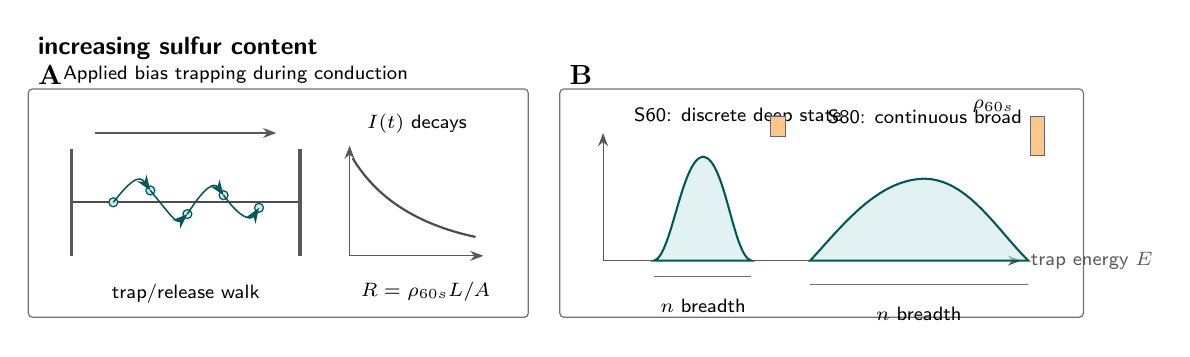
\begin{tikzpicture}[
  font=\sffamily\scriptsize,
  >=Stealth,
  panel/.style={draw=black!55, line width=.45pt, rounded corners=1.5pt},
  axis/.style={black!65, line width=.4pt, -Stealth},
  wire/.style={black!70, line width=.8pt},
  trap/.style={circle, draw=teal!70!black, fill=teal!18, line width=.45pt, inner sep=1.15pt},
  dist/.style={draw=teal!70!black, fill=teal!18, line width=.75pt, fill opacity=.62},
  rho/.style={draw=black!60, fill=orange!45, line width=.35pt}
]

\node[font=\sffamily\bfseries\small, anchor=west] at (0,3.42) {increasing sulfur content};

\begin{scope}
  \node[font=\bfseries, anchor=west] at (0,3.08) {A};
  \node[anchor=west] at (.32,3.08) {Applied bias trapping during conduction};
  \draw[panel] (0,0) rectangle (6.35,2.9);

  \draw[wire] (.55,1.46) -- (3.45,1.46);
  \draw[black!65, line width=1.3pt] (.55,.78) -- (.55,2.14);
  \draw[black!65, line width=1.3pt] (3.45,.78) -- (3.45,2.14);
  \draw[axis] (.85,2.34) -- (3.15,2.34);

  \foreach \x/\y in {1.08/1.46,1.55/1.61,2.02/1.31,2.48/1.55,2.93/1.39}
    \node[trap] at (\x,\y) {};
  \draw[teal!70!black, line width=.55pt, -Stealth] (1.08,1.46) .. controls (1.33,1.78) and (1.42,1.80) .. (1.55,1.61);
  \draw[teal!70!black, line width=.55pt, -Stealth] (1.55,1.61) .. controls (1.79,1.32) and (1.88,1.18) .. (2.02,1.31);
  \draw[teal!70!black, line width=.55pt, -Stealth] (2.02,1.31) .. controls (2.24,1.66) and (2.36,1.72) .. (2.48,1.55);
  \draw[teal!70!black, line width=.55pt, -Stealth] (2.48,1.55) .. controls (2.68,1.27) and (2.82,1.22) .. (2.93,1.39);
  \node[anchor=north] at (2.0,.55) {trap/release walk};

  \draw[axis] (4.08,.78) -- (5.78,.78);
  \draw[axis] (4.08,.78) -- (4.08,2.18);
  \draw[black!70, line width=.8pt] (4.12,2.02) .. controls (4.42,1.52) and (4.93,1.18) .. (5.68,1.02);
  \node[anchor=west] at (4.18,2.46) {$I(t)$ decays};
  \node[anchor=west] at (4.1,.33) {$R=\rho_{60s}L/A$};
\end{scope}

\begin{scope}[xshift=6.75cm]
  \node[font=\bfseries, anchor=west] at (0,3.08) {B};
  \draw[panel] (0,0) rectangle (6.65,2.9);

  \draw[axis] (.55,.72) -- (5.86,.72) node[right] {trap energy $E$};
  \draw[axis] (.55,.72) -- (.55,2.34);

  \draw[dist] (1.2,.72) .. controls (1.42,.78) and (1.55,2.02) .. (1.82,2.04)
    .. controls (2.1,2.02) and (2.2,.78) .. (2.43,.72) -- cycle;
  \draw[dist] (3.18,.72) .. controls (3.58,1.15) and (4.02,1.74) .. (4.62,1.76)
    .. controls (5.18,1.76) and (5.55,1.11) .. (5.95,.72) -- cycle;

  \draw[black!55, line width=.45pt] (1.2,.52) -- (2.43,.52);
  \draw[black!55, line width=.45pt] (3.18,.42) -- (5.95,.42);
  \node[anchor=north] at (1.82,.36) {$n$ breadth};
  \node[anchor=north] at (4.56,.26) {$n$ breadth};

  \node[anchor=west] at (.82,2.55) {S60: discrete deep state};
  \node[anchor=west] at (3.28,2.55) {S80: continuous broad};
  \draw[rho] (2.68,2.3) rectangle (2.86,2.55);
  \draw[rho] (5.98,2.05) rectangle (6.16,2.55);
  \node[anchor=west] at (5.12,2.68) {$\rho_{60s}$};
\end{scope}

\end{tikzpicture}
\end{document}
